\subsection{Modalities}

\begin{figure}
    \centering
    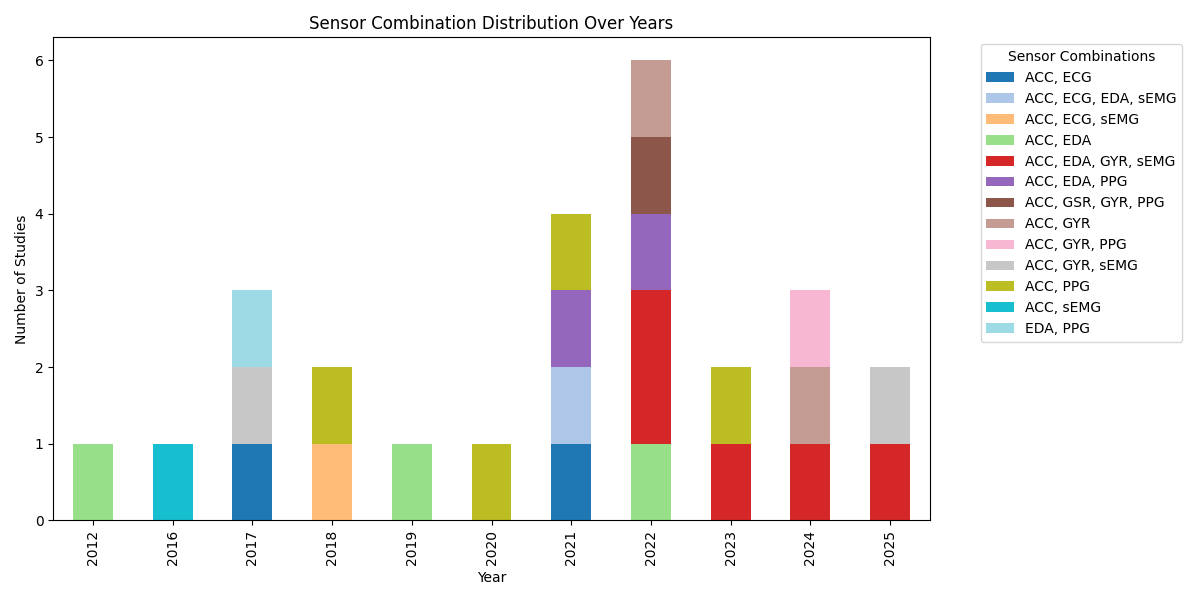
\includegraphics[width=1\textwidth]{Discussion/figures/Sensor_Combination_Distribution_Over_the_Years.png}
    \caption{Sensor combination distribution over the years.}
    \label{fig:sensor_comb_over_years}
\end{figure}

\subsubsection{Detection}
Based on the 26 reviewed articles, it is apparent that non-EEG multimodal sensor configurations for detecting motor seizures are feasible and have a great promise compared to conventional detection and management methods. 

It is important to note that direct comparison across the reviewed studies is challenging due to methodological heterogeneity, differences in study populations, and variability in training datasets. Nevertheless, the ACC + GYR + EDA + sEMG sensor combination performance is consistently high across studies (table \ref{tab:modalities}) regardless to the study setups. This may be because these setups combine the reliability of motion-based detection through ACC, GYR, and sEMG with the stabilizing contribution of physiological signals such as EDA, which helps reduce false alarms and enhance overall performance. Additionally, sEMG has been reported to rapidly detect seizures with notably low detection delay (11.7s) \cite{De_Cooman2018-pq}, highlighting its importance for timely intervention.

ACC + EDA is also one of the top performing combinations, with the advantages of less sensor modalities used to indicate less costs, more easier data pre-processing and signal fusion models. This is perhaps due to EDA’s sensitivity to sympathetic activation which occurs closely with motor seizure onset consistent across multiple studies involving both children and adults \cite{Casanovas_Ortega2022-yx}, in addition to EDA being less sensitive to motion artifacts than other physiological signals like PPG for instance \cite{Ismail2021-fs}, making it more robust. Additionally, studies have demonstrated peri-ictal rises in EDA correlate with postictal generalized EEG suppression (PGES), a known SUDEP risk factor \cite{Barot2019-nx,Regalia2019-ch}, highlighting the potential of EDA in SUDEP prevention.

While this highlights the significance of EDA data in seizure detection, some studies have reported poor performance of EDA as a standalone modality and even when combined with other sensors such as PPG or ACC \cite{Yu2023-ss,Tang2021-td}. This variability across studies stems perhaps from the age-related variability in EDA signals reported by the pediatric study \cite{Ge2023-ab}, highlighting the need for algorithms trained on EDA to count for such variability. 

Other physiological sensors such as PPG have also been widely used to extract biomarkers including HR \cite{Cogan2017-lg,Nasseri2021-xn,Vakilna2024-hk,Xu2022-tx,Jiang2022-zu,Arends2018-ew}, HRV \cite{Vakilna2024-hk,Jiang2022-zu}, SpO2 \cite{Cogan2017-lg}, and BVP \cite{Yu2023-ss,Nasseri2021-xn,Tang2021-td}. Among these, BVP in particular has shown strong potential, consistently achieving high performance across seizure types. This is consistent with findings from the observational clinical study conducted by Mohammadpour Touserkani et al. \cite{Mohammadpour_Touserkani2020-tk}, where not only heart rate–dependent variables (frequency), but also other features of the PPG signal such as smoothness and slope were shown to vary relative to seizure timing. These additional PPG-derived features contribute to the improved ability of BVP-based detection algorithms to accurately identify seizures beyond the sole use of heart rate metrics, highlighting the superior seizure discriminative information contained in BVP signals.

ECG has also been employed to derive HR \cite{Hegarty-Craver2021-hk,De_Cooman2018-pq,Van_Andel2017-yx} and HRV \cite{Hegarty-Craver2021-hk}, with some studies reporting that unimodal ECG systems can achieve performance comparable to multimodal approaches \cite{Hegarty-Craver2021-hk,De_Cooman2018-pq}. However, ECG w as used less frequently in the reviewed studies, largely due to its susceptibility to motion artifacts \cite{Van_Andel2017-yx}, its relative impracticality as a wearable sensor (requiring multiple electrodes to be placed on the chest or limbs), and the high inter-patient variability observed in cardiac-derived signals \cite{Van_Andel2017-yx,De_Cooman2018-pq}.

Because of these limitations, ECG has mostly been used in nocturnal studies \cite{De_Cooman2018-pq,Van_Andel2017-yx}. This is relevant since SUDEP is more likely to happen at night \cite{Friedman2022-mo}, and HR and HRV are under investigation as potential SUDEP   biomarkers \cite{Barot2019-nx}. Thus, ECG may serve a dual role in seizure detection and monitoring SUDEP-related autonomic changes.

Some studies have also investigated the use of non-traditional biomarkers for seizure detection, and interestingly, several of these have demonstrated detection capabilities comparable to, or even exceeding, those of more established biomarkers. Hamlin et al. \cite{Hamlin2021-sd} investigated the incorporation of audio features, derived from a MIC, in the detection system and reported that audio signals proved to be among the top ten features establishing separability between seizure and non-seizure data in four or five patients. Wang et al. \cite{Wang2025-ql} investigated the incorporation of attitude angle signals  like pitch or roll in their detection system and reported that in multimodal combinations, adding pitch or roll alongside or replacing ACC, GYR outperformed combinations that excluded them across all models, as attitude signals were shown to have better anti-interference ability i.e. the attitude angle signals didn’t show a wide range of energy enhancements compared to ACC and GYR in non-seizure periods.  Instead of using raw ACC data, Xu et al. \cite{Xu2022-tx} used NOWM to distinguish seizure-like activity from normal daily movements.

In addition to the type of used modalities, sensor placement and signal quality were found to substantially impact detection performance. Tang et al. \cite{Tang2021-td}, for example, collected signals from different body parts, which introduced inconsistency in signal acquisition. Arends et al. \cite{Arends2018-ew} had to exclude individuals with abnormal movements or darker skin tones, as PPG signal quality was strongly affected by light intensity. Similarly, the chest-worn sensor used in Hegarty-Craver et al. \cite{Hegarty-Craver2021-hk} was not optimal for detecting limb movements, reducing the device’s overall sensitivity. Cogan et al. \cite{Cogan2017-lg} also reported issues of missing data during recordings caused by the SpO$_2$ sensor.

Thus, future studies should validate the incorporation of these biomarkers into detection systems, while also assessing optimal sensor placement. Evidence from \cite{Milosevic2016-ee,De_Cooman2018-pq} shows that different sensor placements produce different outcomes, highlighting the importance of placement as a design consideration. In addition, studies should account for the variability exhibited by physiological signals across different populations by increasing and diversifying their cohorts, and by developing personalized models for highly patient-dependent modalities such as HR and HRV.

\subsubsection{Prediction and Forecasting}
Although the tasks and methodological scopes of the three studies varied, together they provide strong evidence for the feasibility of using wearable data from the Empatica E4 wristband in combination with machine learning or deep learning algorithms for seizure prediction and forecasting. Vieluf et al. \cite{Vieluf2023-ta,Vieluf2023-zv} demonstrated that the purely autonomic sensor set of EDA and PPG (from which HR and HRV are derived) could successfully discriminate pre-ictal periods in a substantial proportion of patients in their cohorts. However, the highest prediction performance was reported by Meisel et al. \cite{Meisel2020-ii}, where all available sensor modalities on the E4 device (EDA, PPG/BVP, ACC, and TEMP) were incorporated into the forecasting models, confirming the superiority of multimodal combinations demonstrated in detection studies. 

Biomarkers derived from PPG appear to be the primary seizure detectors, and while two studies \cite{Vieluf2023-ta,Vieluf2023-zv} proposed HR information to have seizure predictive information, the observational clinical study by Mohammadpour Touserkani et al. \cite{Mohammadpour_Touserkani2020-tk} show that frequency, smoothness, and slope change during the peri-ictal and post-ictal phases of a seizure, indicating that raw PPG signals may provide additional information regarding usability of these signals for seizure prediction. Future studies should test raw PPG signals instead of its derived biomarkers in larger and more diverse cohorts.